\documentclass[onlymath]{beamer}

% Think backwards: what do you want people to remember from your talk?
% Don’t say everything.
% Simplify.

\setbeamertemplate{navigation symbols}{}%remove navigation symbols
\setbeamercolor{normal text}{fg=white,bg=black!90}
\setbeamercolor{structure}{fg=white}
\setbeamercolor{alerted text}{fg=red!85!black}
\setbeamercolor{item projected}{use=item,fg=black,bg=item.fg!35}
\setbeamercolor*{palette primary}{use=structure,fg=structure.fg}
\setbeamercolor*{palette secondary}{use=structure,fg=structure.fg!95!black}
\setbeamercolor*{palette tertiary}{use=structure,fg=structure.fg!90!black}
\setbeamercolor*{palette quaternary}{use=structure,fg=structure.fg!95!black,bg=black!80}
\setbeamercolor*{frametitle}{fg=blue!40}
\setbeamercolor*{framesubtitle}{fg=blue!30}
\setbeamercolor*{block title}{parent=structure,bg=black!60}
\setbeamercolor*{block body}{fg=black,bg=black!10}
\setbeamercolor*{block title alerted}{parent=alerted text,bg=black!15}
\setbeamercolor*{block title example}{parent=example text,bg=black!15}
\usefonttheme{serif}

\usepackage{listings}
\usepackage[english]{babel}
\usepackage[utf8]{inputenc}
\usepackage{amsmath}
\usepackage{graphicx}
\usepackage{helvet}

\usepackage{tikz}
\usetikzlibrary{fadings}

\title[{Nopol: Repairing Bugs in Conditional Expressions}]{Nopol: Repairing~Bugs~in~Conditional~Expressions}
\author[Favio DeMarco]{Favio~DeMarco}
\institute[U.B.A. - INRIA]{Universidad de Buenos Aires - INRIA}
\date{\today}
\subject{Computational Sciences}

\begin{document}

  \frame
  {
\begin{quote}
    Take nothing on its looks; take everything on evidence. There's no better rule.
\end{quote}    
– Charles Dickens, ``Great Expectations.''
  }

\frame
  {
  \begin{center}
  
\includegraphics[width=7em]{logofcen}
  \end{center}
    \titlepage
  }

\begin{frame}  
\frametitle{Bugs?}
\begin{quotation}
The difference between the right word and the almost right word is the difference between lightning and a lightning bug.
\end{quotation}
-- Mark Twain
\end{frame}
 
\begin{frame}
\frametitle{Motivation}
\framesubtitle{The Six Stages of Debugging}
\begin{enumerate}
\item  That can’t happen.
\item  That doesn’t happen on my machine.
\item  That shouldn’t happen.
\item  Why does that happen?
\item  Oh, I see.
\item  How did that ever work?
\end{enumerate}
\end{frame}

 
 
\begin{frame}[fragile]
\frametitle{What are conditional expression bugs?}
\begin{lstlisting}[escapeinside=\[\]]
[\textbf{boolean expression}] ? someValue : someOtherValue;

if ([\textbf{boolean expression}]) {
...
}
\end{lstlisting}
\end{frame}

\begin{frame}[fragile]
\frametitle{Change of If Condition Expression (IF-CC)}
Kai Pan et al.\footnote{Toward an understanding of bug fix patterns}:
\begin{quotation}
This bug fix change fixes the bug by changing the condition expression of an if
condition. The previous code has a bug in the if condition logic.
\end{quotation}

\vspace{1em}

\begin{lstlisting}
- if (getView().countSelected() == 0) {
+ if (getView().countSelected() <= 1) {
\end{lstlisting}
\end{frame}
  
\begin{frame}[fragile]
\frametitle{What are conditional expression bugs?}
\framesubtitle{Commons Math - MathUtils class}
    
\begin{lstlisting}[escapeinside=\[\]]
411: public static int gcd(int u, int v) {
412:   if ([\textbf{u * v == 0}]) {
413:     return (Math.abs(u) + Math.abs(v));
414:   }
...
\end{lstlisting}

\vspace{2em}

\centering What about \texttt{u=0x00110000} and  \texttt{v=0x01100000}?

\end{frame}

\begin{frame}
\frametitle{Problem I}
\framesubtitle{How does the tool know something is \textit{wrong}?}
\begin{center}
\Huge{404}
\end{center}
\end{frame}

\begin{frame}
\frametitle{Problem I}
\framesubtitle{How does the tool know something is \textit{wrong}?}
Some kind of specification:
\begin{itemize}
 \item Model
 \item Contracts
 \item \textbf{Unit tests}
 \item \dots
\end{itemize}
\end{frame}

\begin{frame}[fragile]
\frametitle{How does the tool know something is \textit{wrong}?}
\framesubtitle{At least one failing test}
      
      \begin{lstlisting}[escapeinside=\[\]]
assertEquals([\textbf{3 * (1$<<$15)}]
            , gcd(3 * (1<<20), 9 * (1<<15)));
	\end{lstlisting}
\end{frame}

\begin{frame}
\frametitle{No-Pol input}
\begin{itemize}
 \item Java source code.
 \item Unit tests with at least one failing test case.
 \item Dependencies (\textit{classpath}).
\end{itemize}
\end{frame}

\begin{frame}
\frametitle{No-Pol output}
Patched Java source file.
\end{frame}


\frame
{
    \frametitle{Overview}
    \framesubtitle{Trial and error}
  \begin{center}
  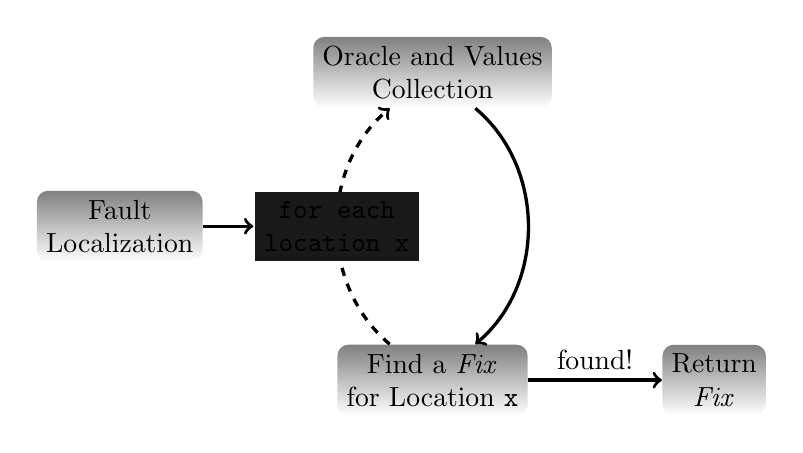
\begin{tikzpicture}[
  every matrix/.style={ampersand replacement=\&,column sep=4em,row sep=3em},
  box/.style={rounded corners,fill=gray,path fading=south},
  flow/.style={->, very thick},
  fail/.style={->, very thick, dashed},
  every node/.style={align=center}]
  
% Position the nodes using a matrix layout
\matrix{

      \& \node[box] (test) {Oracle and Values \\ Collection};
      \& \\
      \node[box] (faultLocalization) {Fault \\ Localization};
      \& \\
      \& \node[box] (generateCandidate) {Find a \textit{Fix} \\ for Location \texttt{x}};
      \& \node[box] (output) {Return \\ \textit{Fix}};
      \\
  };

% Draw the arrows between the nodes and label them.
\draw [flow] (test) to[bend left=50] (generateCandidate);
\draw [flow] (generateCandidate) to node[above] {found!} (output);
\draw [fail] (generateCandidate) to[bend left=50] node[font=\ttfamily, fill=black!90] (statement) {for each \\ location x} (test);
\draw [flow] (faultLocalization) -- (statement.west);

\end{tikzpicture}

  \end{center}
}


\begin{frame}
\frametitle{Problem II}
\framesubtitle{Where is the bug?}
  \begin{center}
  
\includegraphics[width=.8\paperwidth]{WheresWally}
  \end{center}
\end{frame}

\begin{frame}[fragile]
    \frametitle{Fault Localization (statement ranking)}
      \framesubtitle{GZoltar - Ochiai coefficient}
The suspiciousness $s_j$ of a statement $j$ depends on:
\begin{itemize}
 \item The number of \textbf{failing} test cases \textbf{executing} statement $j$ 
 \item The number of \textbf{failing} test cases \textbf{not executing} statement $j$
 \item The number of \textbf{successful} tests \textbf{executing} statement $j$
\end{itemize}
\end{frame}


\begin{frame}[fragile]
\frametitle{Fault Localization (statement ranking)}
\framesubtitle{GZoltar - Ochiai coefficient}
\begin{verbatim}
MathUtils:413 - Suspiciousness: 0.23570226039551587
MathUtils:431 - Suspiciousness: 0.1543033499620919
\end{verbatim}
\dots
\begin{verbatim}
MathUtils:460 - Suspiciousness: 0.11322770341445956
MathUtils:412 - Suspiciousness: 0.11180339887498948
\end{verbatim}
\dots
\end{frame}


\begin{frame}[fragile]
\frametitle{Fault Localization (statement ranking)}
\framesubtitle{GZoltar - Ochiai coefficient}
\begin{verbatim}
...
MathUtils:460 - Suspiciousness: 0.11322770341445956
MathUtils:412 - Suspiciousness: 0.11180339887498948
...
\end{verbatim}

\begin{lstlisting}[escapeinside=\[\]]
411: public static int gcd(int u, int v) {
412:   if ([\textbf{u * v == 0}]) {
413:     return (Math.abs(u) + Math.abs(v));
414:   }
\end{lstlisting}
\end{frame}


\frame
{
  \frametitle{Oracle and Values Collection}
  \framesubtitle{For Location \texttt{x}}
  \begin{center}
  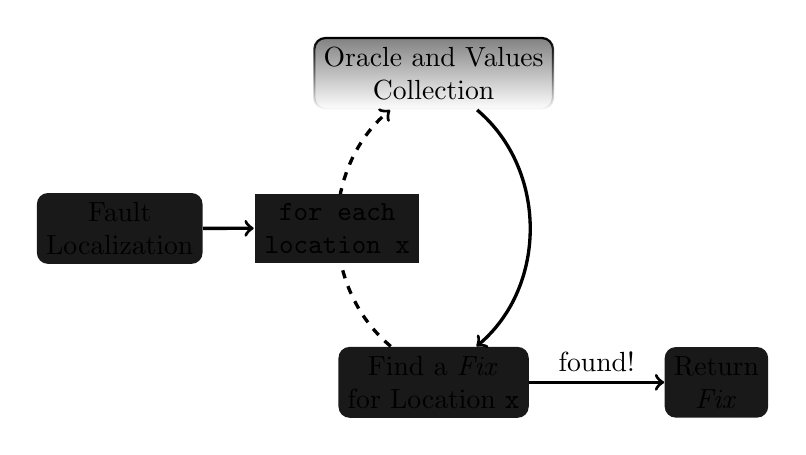
\begin{tikzpicture}[
  every matrix/.style={ampersand replacement=\&,column sep=4em,row sep=3em},
  box/.style={rounded corners,fill=gray,path fading=south, draw, thick},
  shadedbox/.style={rounded corners,fill=black!90},
  flow/.style={->, very thick},
  fail/.style={->, very thick, dashed},
  every node/.style={align=center}]
  
% Position the nodes using a matrix layout
\matrix{

      \& \node[box] (test) {Oracle and Values \\ Collection};
      \& \\
      \node[shadedbox] (faultLocalization) {Fault \\ Localization};
      \& \\
      \& \node[shadedbox] (generateCandidate) {Find a \textit{Fix} \\ for Location \texttt{x}};
      \& \node[shadedbox] (output) {Return \\ \textit{Fix}};
      \\
  };

% Draw the arrows between the nodes and label them.
\draw [flow] (test) to[bend left=50] (generateCandidate);
\draw [flow] (generateCandidate) to node[above] {found!} (output);
\draw [fail] (generateCandidate) to[bend left=50] node[font=\ttfamily, fill=black!90] (statement) {for each \\ location x} (test);
\draw [flow] (faultLocalization) -- (statement.west);

\end{tikzpicture}

  \end{center}
}

\frame
{
  \frametitle{Oracle and Values Collection}
  \framesubtitle{For Location \texttt{x}}
  Two steps:
  \begin{center}
  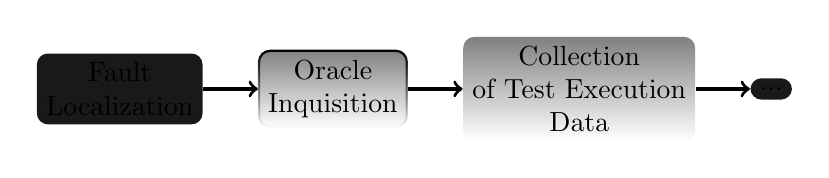
\begin{tikzpicture}[
  every matrix/.style={ampersand replacement=\&,column sep=2em,row sep=2em},
  shadedbox/.style={rounded corners,fill=black!90},
  nobox/.style={rounded corners,fill=gray,path fading=south},
  box/.style={nobox, draw, thick},
  flow/.style={->, very thick},
  fail/.style={->, thick, dashed},
  every node/.style={align=center}]
  
% Position the nodes using a matrix layout
\matrix{
    \node[shadedbox] (faultLocalization) {Fault \\ Localization};
    \& \node[box] (oracleInquisition) {Oracle \\ Inquisition};
    \& \node[nobox] (collectionOfTestExecutionData) {Collection \\ of Test Execution \\ Data};
    \& \node[shadedbox] (empty) {...};
    \\
  };

% Draw the arrows between the nodes and label them.
\draw [flow] (faultLocalization) -- (oracleInquisition);
\draw [flow] (oracleInquisition) -- (collectionOfTestExecutionData);
\draw [flow] (collectionOfTestExecutionData) -- (empty);

\end{tikzpicture}

  \end{center}
}

\begin{frame}
  \frametitle{Oracle Inquisition}
  \framesubtitle{For Location \texttt{x}}
 \begin{equation*}
  \texttt{if(}\overbrace{\texttt{a < b}}^{\displaystyle \textsf{bug}}\texttt{)} \qquad \underbrace{\begin{array}{cc}
                                         \texttt{if(true)} \quad & \quad \texttt{if(false)} \\
                                         PASS \quad & \quad KO
                                        \end{array} }_{\displaystyle \textsf{Oracle}}
 \end{equation*}
\end{frame}

\frame
{
  \frametitle{Collection of Test Execution Data}
  \framesubtitle{For Location \texttt{x}}
  \begin{center}
  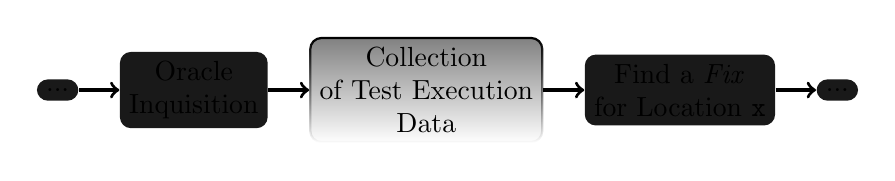
\begin{tikzpicture}[
  every matrix/.style={ampersand replacement=\&,column sep=1.5em},
  box/.style={rounded corners,fill=gray,path fading=south, draw, thick},
  shadedbox/.style={rounded corners,fill=black!90},
  flow/.style={->, very thick},
  fail/.style={->, thick, dashed},
  every node/.style={align=center}]
  
% Position the nodes using a matrix layout
\matrix{
    \node[shadedbox] (empty1) {...};
    \& \node[shadedbox] (oracleInquisition) {Oracle \\ Inquisition};
    \& \node[box] (collectionOfTestExecutionData) {Collection \\ of Test Execution \\ Data};
    \& \node[shadedbox] (constraintsGeneration) {Find a \textit{Fix} \\ for Location \texttt{x}};
    \& \node[shadedbox] (empty2) {...};
    \\
  };

% Draw the arrows between the nodes and label them.
\draw [flow] (empty1) -- (oracleInquisition);
\draw [flow] (oracleInquisition) -- (collectionOfTestExecutionData);
\draw [flow] (collectionOfTestExecutionData) -- (constraintsGeneration);
\draw [flow] (constraintsGeneration) -- (empty2);

\end{tikzpicture}

  \end{center}
}


\begin{frame}[fragile]
  \frametitle{Collection of Test Execution Data}
  \framesubtitle{For Location \texttt{x}}
\begin{lstlisting}[basicstyle=\footnotesize]
 42: public static final double TWO_PI = 2 * FastMath.PI;
...
411: public static int gcd(int u, int v) {
412:   if (u * v == 0) {
413:     return (Math.abs(u) + Math.abs(v));
414:   }
\end{lstlisting}

\begin{center}
\begin{tabular}{|l|l|l|l|l}
\hline
 & \texttt{TWO\_PI} & \texttt{u} & \texttt{v} & \\
\hline
\textit{testZero} & 6.283185\dots & 0 & 0 & \\
\hline
\textit{testOverflow} & 6.283185\dots & 0x00110000 & 0x01100000 & \\
\hline
 & & & & \\
\end{tabular}
\end{center}
\end{frame}


\frame
{
  \frametitle{Find a \textit{Fix}}
  \framesubtitle{For Location \texttt{x}}
  \begin{center}
  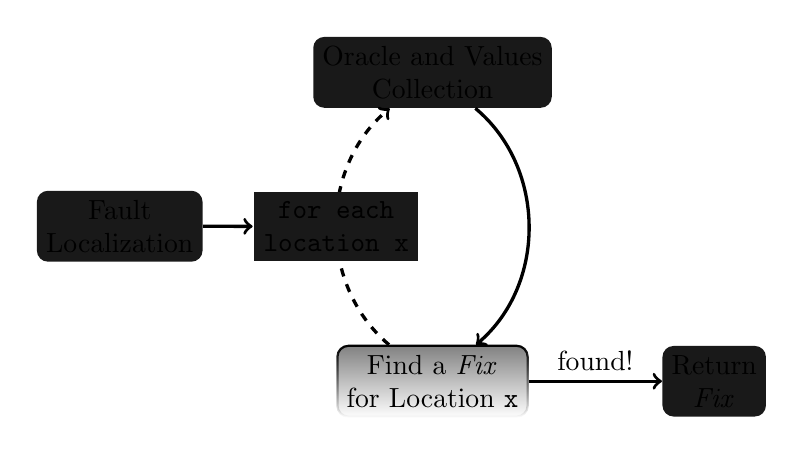
\begin{tikzpicture}[
  every matrix/.style={ampersand replacement=\&,column sep=4em,row sep=3em},
  box/.style={rounded corners,fill=gray,path fading=south, draw, thick},
  shadedbox/.style={rounded corners,fill=black!90},
  flow/.style={->, very thick},
  fail/.style={->, very thick, dashed},
  every node/.style={align=center}]
  
% Position the nodes using a matrix layout
\matrix{

      \& \node[shadedbox] (test) {Oracle and Values \\ Collection};
      \& \\
      \node[shadedbox] (faultLocalization) {Fault \\ Localization};
      \& \\
      \& \node[box] (generateCandidate) {Find a \textit{Fix} \\ for Location \texttt{x}};
      \& \node[shadedbox] (output) {Return \\ \textit{Fix}};
      \\
  };

% Draw the arrows between the nodes and label them.
\draw [flow] (test) to[bend left=50] (generateCandidate);
\draw [flow] (generateCandidate) to node[above] {found!} (output);
\draw [fail] (generateCandidate) to[bend left=50] node[font=\ttfamily, fill=black!90] (statement) {for each \\ location x} (test);
\draw [flow] (faultLocalization) -- (statement.west);

\end{tikzpicture}

  \end{center}
}

\frame
{
  \frametitle{Constraints Generation (aka secret sauce)}
  \framesubtitle{For Location \texttt{x}}
  \begin{center}
  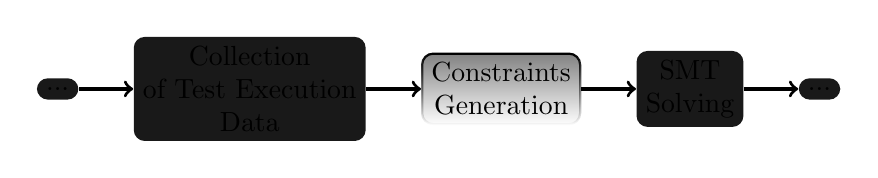
\begin{tikzpicture}[
  every matrix/.style={ampersand replacement=\&,column sep=2em,row sep=2em},
  box/.style={rounded corners,fill=gray,path fading=south, draw, thick},
  shadedbox/.style={rounded corners,fill=black!90},
  flow/.style={->, very thick},
  fail/.style={->, thick, dashed},
  every node/.style={align=center}]
  
% Position the nodes using a matrix layout
\matrix{
    \node[shadedbox] (empty1) {...};
    \& \node[shadedbox] (collectionOfTestExecutionData) {Collection \\ of Test Execution \\ Data};
    \& \node[box] (constraintsGeneration) {Constraints \\ Generation};
    \& \node[shadedbox] (smtSolving) {SMT \\ Solving};
    \& \node[shadedbox] (empty2) {...};
    \\
  };

% Draw the arrows between the nodes and label them.
\draw [flow] (empty1) -- (collectionOfTestExecutionData);
\draw [flow] (collectionOfTestExecutionData) -- (constraintsGeneration);
\draw [flow] (constraintsGeneration) -- (smtSolving);
\draw [flow] (smtSolving) -- (empty2);

\end{tikzpicture}

  \end{center}
}

\begin{frame}
  \frametitle{Constraints Generation}
  \framesubtitle{Oracle-Guided Component-Based Program Synthesis:}
  Components and line numbers:
\begin{align*}
\textsf{Constants} & \left\{ \begin{array}{ll}
        0 & \texttt{true} \\
        1 & \texttt{false} \\
        2 & \texttt{-1} \\
        3 & \texttt{0} \\
        4 & \texttt{1}
    \end{array}\right. \\
\textsf{Input values} & \left\{ \begin{array}{lllll}
        5 & \texttt{u} & &		8 & \texttt{col != null} \\
        6 & \texttt{v} & &		9 & \texttt{col.isEmpty()} \\
        7 & \texttt{TWO\_PI} & &	10 & \texttt{col.size()} \\
        \dots
    \end{array}\right. \\
\textsf{Oracle} & \left\{ \begin{array}{ll}
        l_O &  \textsf{Expected} \\
            & \textsf{output}
    \end{array}\right.
\end{align*}
\end{frame}

% \begin{frame}
% conditions to meet by the solution
% \end{frame}

\begin{frame}
  \frametitle{Constraints Generation}
  \framesubtitle{Oracle-Guided Component-Based Program Synthesis:}
  Components and line numbers:
  
\begin{align*}
l_{O1} & = l_{I11} < l_{I12} \\
l_{O2} & = l_{I21} <= l_{I22} \\ 
l_{O3} & = l_{I31} + l_{I32} \\
l_{O4} & = l_{I41} * l_{I42} \\
l_{O5} & = l_{I51} \wedge l_{I52} \\
& ... \\
l_{On} & = l_{In1} ? l_{In2} : l_{In3}
\end{align*}
\end{frame}

\begin{frame}[fragile]
  \frametitle{Constraints Generation}
  \framesubtitle{Example}
  Components:
\begin{verbatim}
0   I
lO  oracle
lO1 := f1(lI1);
lO2 := f2(lI2_1, lI2_2);
\end{verbatim}
An answer:
\begin{verbatim}
lI1 = 1    lO1 = 2
lI2_1 = 0  lO2 = 1
lI2_2 = 0  lO  = 2
\end{verbatim}
\end{frame}

\begin{frame}[fragile]
  \frametitle{Constraints Generation}
  \framesubtitle{Example}
\begin{columns}
\column{.5\textwidth}
  Components:
\begin{verbatim}
0   I
lO  oracle
lO1 := f1(lI1);
lO2 := f2(lI2_1, lI2_2);
\end{verbatim}
An answer:
\begin{verbatim}
lI1 = 1    lO1 = 2
lI2_1 = 0  lO2 = 1
lI2_2 = 0  lO  = 2
\end{verbatim}
\column{.5\textwidth}
Another representation:
\begin{verbatim}
0 I
1 := f2(0, 0);
return f1(1);
\end{verbatim}
What it means:
\begin{verbatim}
f(I) = f1(f2(I, I));
\end{verbatim}
\end{columns}
\end{frame}

\begin{frame}[fragile]
  \frametitle{Constraints Generation}
  \framesubtitle{Example}
  Well formed program:
\begin{columns}
\column{.5\textwidth}
\begin{verbatim}
0   I
lO  oracle
lO1 := f1(lI1);
lO2 := f2(lI2_1, lI2_2);
\end{verbatim}
\column{.5\textwidth}
\begin{itemize}
 \item all line numbers should be between 0 and 3.
 \item the output lines should be greater than the input lines (acyclicity).
 \item \texttt{lO1} $\neq$ \texttt{lO2} (consistency)
\end{itemize}
\end{columns}
\end{frame}

\begin{frame}
  \frametitle{Constraints Generation}
  \framesubtitle{Example}
Library:
\begin{align*}
O_{1} & = f_{1}(I_1) \\
O_{2} & = f_{2}(I_{21}, I_{22}) \\ 
\end{align*}
\end{frame}

\begin{frame}[fragile]
  \frametitle{Constraints Generation}
  \framesubtitle{Example}
Connectivity:
\begin{columns}
\column{.5\textwidth}
\begin{verbatim}
0   I
lO  oracle
lO1 := f1(lI1);
lO2 := f2(lI2_1, lI2_2);
\end{verbatim}
\column{.5\textwidth}
\begin{itemize}
 \item if $I_{21} = I$ then $l_{I21} = 0$
 \item if $I_{1} = O_2$ then $l_{I1} = l_{O2}$
\end{itemize}
\end{columns}
\end{frame}


\frame
{
  \frametitle{Constraints Generation}
  \framesubtitle{Oracle-Guided Component-Based Program Synthesis}
\begin{align*}
\phi_{func}(L, I, O) = \exists P, R & \psi_{wfp}(L) \\
& \wedge \psi_{lib}(P, R)  \\ 
& \wedge \psi_{conn}(L, I, O, P, R)
\end{align*}
}


\frame
{
  \frametitle{Constraints Generation}
  \framesubtitle{Oracle-Guided Component-Based Program Synthesis}
\begin{align*}
\psi_{wfp}(L) = & \bigwedge_{x \in P} (0 \leq l_x < M) \\
& \wedge \bigwedge_{x \in R} (|I| \leq l_x < M) \\
& \wedge \psi_{cons}(L) \wedge \psi_{acyc}(L)
\end{align*}
}

\frame
{
  \frametitle{Constraints Generation}
  \framesubtitle{Oracle-Guided Component-Based Program Synthesis}
\begin{equation*}
\psi_{lib}(P, R) = \left( \bigwedge^N_{i=1} \phi_i(I_i, O_i) \right)
\end{equation*}

\begin{equation*}
\psi_{conn}(L, I, O, P, R) = \bigwedge_{x, y \in P \cup R \cup I \cup \{O\}} (l_x = l_y \Rightarrow x = y)
\end{equation*}
}


% \begin{frame}
% Slide sobre levels
% \end{frame}


 \begin{frame}[fragile]
    \frametitle{Preconditions bugs}
      \framesubtitle{Commons Collections - SequencedHashMap class}
\begin{lstlisting}
private Entry findEntry(Map.Entry e) {
  if (e == null)
    return null;
  Entry entry = entries.get(e.getKey());
  if (entry.equals(e)) // entry can be null
    return entry;
  else
    return null;
}
\end{lstlisting}
\end{frame}

\begin{frame}[fragile]
\frametitle{Addition of Precondition Check (IF-APC)}
Kai Pan et al.\footnote{Toward an understanding of bug fix patterns}:
\begin{quotation}
This bug fix adds an if predicate to ensure a precondition is met before an
object is accessed or an operation is performed.
\end{quotation}

\vspace{1em}

\begin{lstlisting}[basicstyle=\scriptsize]
- lastChunk.init(seg,expander,x,styles,

-   fontRenderContext, context.rules.getDefault());

+ if (!lastChunk.initialized)

+   lastChunk.init(seg,expander,x,styles,

+     fontRenderContext, context.rules.getDefault());
\end{lstlisting}
\end{frame}

  \frame
  {
    \frametitle{Problems}
\begin{itemize}
\item It won't work with infinite loop bugs.
\item Can't automate the testing process.
\item It's not easy to find candidates.
\end{itemize}    
  }

  \frame
  {
    \frametitle{Problems}
    \framesubtitle{Test quality}
   \begin{quote}
    Quality is free, but only to those who are willing to pay heavily for it.
   \end{quote}
    Tom DeMarco, Peopleware   
  }
  
  \frame
  {
    \frametitle{Limitations}
    \framesubtitle{Test quality}
\begin{itemize}
\item Only 1 set of input values.
\item Branch coverage.
\item A \textit{removed} precondition can generate an infinite loop.
\item Tests that exercise both branches.
\item Generates \textit{a} fix not \textbf{THE} fix.
\end{itemize}        
  }

  \frame
  {  
    \frametitle{Contributions}
      \framesubtitle{Process}
\begin{itemize}
\item Statement ranking (GZoltar)  $\rightarrow$
\item Ad hoc code manipulation and values capturing $\rightarrow$
\item Repair Constraint  $\rightarrow$
\item Program Synthesis (OGCBPS\footnote{Oracle-Guided Component-Based Program Synthesis} -paper-)
\end{itemize}
}


  \frame
  {
    \frametitle{Experimental methodology}
    Seeded and wild bugs.
  }
  
  \frame
  {
    \frametitle{Evaluation / Validation}
    Generated patches vs. reality.
  }
  
  \frame
  {
    \frametitle{Perspectives}
    
  }
  
  \frame
  {
    \frametitle{Conclusion}
    
  }

  \frame
  {
    \frametitle{Contribution}
    
  }
  
 \begin{frame}[fragile]
    \frametitle{Case study}
      \framesubtitle{Commons Math - MathUtils class}
\begin{lstlisting}[escapeinside=\[\]]
411: public static int gcd(int u, int v) {
412:   if ([\textbf{u * v == 0}]) {
413:     return (Math.abs(u) + Math.abs(v));
414:   }
...
\end{lstlisting}
\end{frame}

 \begin{frame}[fragile]
    \frametitle{Case study}
      \framesubtitle{Commons Math}
        \begin{lstlisting}[escapeinside=\[\]]
assertEquals([\textbf{3 * (1$<<$15)}]
        , gcd(3 * (1<<20), 9 * (1<<15)));
	\end{lstlisting}
\end{frame}

 \begin{frame}[fragile]
    \frametitle{Case study}
      \framesubtitle{Statement ranking (GZoltar)}
\begin{verbatim}
MathUtils:413 Suspiciousness 0.23570226039551587
MathUtils:431 Suspiciousness 0.1543033499620919
\end{verbatim}
\dots
\begin{verbatim}
MathUtils:460 Suspiciousness 0.11322770341445956
MathUtils:412 Suspiciousness 0.11180339887498948
\end{verbatim}
\end{frame}

 \begin{frame}[fragile]
    \frametitle{Case study}
      \framesubtitle{Ad hoc code manipulation and values capturing (OGCBPS -paper-)}
\begin{lstlisting}[escapeinside=\[\]]
411: public static int gcd(int u, int v) {
412:   if ([\textbf{true}]) {
413:     return (Math.abs(u) + Math.abs(v));
414:   }
...
\end{lstlisting}
\end{frame}

 \begin{frame}[fragile]
    \frametitle{What are conditional bugs?}
    \framesubtitle{Commons Math - MathUtils class}
        \begin{lstlisting}[escapeinside=\[\]]
public static int gcd(int u, int v) {
    if ([\textbf{(u == 0) $||$ (v == 0)}]) {
        return (Math.abs(u) + Math.abs(v));
    }
    // ...
}
	\end{lstlisting}
\end{frame}

\end{document}
